\documentclass[twoside]{book}

% Packages required by doxygen
\usepackage{fixltx2e}
\usepackage{calc}
\usepackage{doxygen}
\usepackage[export]{adjustbox} % also loads graphicx
\usepackage{graphicx}
\usepackage[utf8]{inputenc}
\usepackage{makeidx}
\usepackage{multicol}
\usepackage{multirow}
\PassOptionsToPackage{warn}{textcomp}
\usepackage{textcomp}
\usepackage[nointegrals]{wasysym}
\usepackage[table]{xcolor}

% Font selection
\usepackage[T1]{fontenc}
\usepackage[scaled=.90]{helvet}
\usepackage{courier}
\usepackage{amssymb}
\usepackage{sectsty}
\renewcommand{\familydefault}{\sfdefault}
\allsectionsfont{%
  \fontseries{bc}\selectfont%
  \color{darkgray}%
}
\renewcommand{\DoxyLabelFont}{%
  \fontseries{bc}\selectfont%
  \color{darkgray}%
}
\newcommand{\+}{\discretionary{\mbox{\scriptsize$\hookleftarrow$}}{}{}}

% Page & text layout
\usepackage{geometry}
\geometry{%
  a4paper,%
  top=2.5cm,%
  bottom=2.5cm,%
  left=2.5cm,%
  right=2.5cm%
}
\tolerance=750
\hfuzz=15pt
\hbadness=750
\setlength{\emergencystretch}{15pt}
\setlength{\parindent}{0cm}
\setlength{\parskip}{3ex plus 2ex minus 2ex}
\makeatletter
\renewcommand{\paragraph}{%
  \@startsection{paragraph}{4}{0ex}{-1.0ex}{1.0ex}{%
    \normalfont\normalsize\bfseries\SS@parafont%
  }%
}
\renewcommand{\subparagraph}{%
  \@startsection{subparagraph}{5}{0ex}{-1.0ex}{1.0ex}{%
    \normalfont\normalsize\bfseries\SS@subparafont%
  }%
}
\makeatother

% Headers & footers
\usepackage{fancyhdr}
\pagestyle{fancyplain}
\fancyhead[LE]{\fancyplain{}{\bfseries\thepage}}
\fancyhead[CE]{\fancyplain{}{}}
\fancyhead[RE]{\fancyplain{}{\bfseries\leftmark}}
\fancyhead[LO]{\fancyplain{}{\bfseries\rightmark}}
\fancyhead[CO]{\fancyplain{}{}}
\fancyhead[RO]{\fancyplain{}{\bfseries\thepage}}
\fancyfoot[LE]{\fancyplain{}{}}
\fancyfoot[CE]{\fancyplain{}{}}
\fancyfoot[RE]{\fancyplain{}{\bfseries\scriptsize Generated by Doxygen }}
\fancyfoot[LO]{\fancyplain{}{\bfseries\scriptsize Generated by Doxygen }}
\fancyfoot[CO]{\fancyplain{}{}}
\fancyfoot[RO]{\fancyplain{}{}}
\renewcommand{\footrulewidth}{0.4pt}
\renewcommand{\chaptermark}[1]{%
  \markboth{#1}{}%
}
\renewcommand{\sectionmark}[1]{%
  \markright{\thesection\ #1}%
}

% Indices & bibliography
\usepackage{natbib}
\usepackage[titles]{tocloft}
\setcounter{tocdepth}{3}
\setcounter{secnumdepth}{5}
\makeindex

% Hyperlinks (required, but should be loaded last)
\usepackage{ifpdf}
\ifpdf
  \usepackage[pdftex,pagebackref=true]{hyperref}
\else
  \usepackage[ps2pdf,pagebackref=true]{hyperref}
\fi
\hypersetup{%
  colorlinks=true,%
  linkcolor=blue,%
  citecolor=blue,%
  unicode%
}

% Custom commands
\newcommand{\clearemptydoublepage}{%
  \newpage{\pagestyle{empty}\cleardoublepage}%
}

\usepackage{caption}
\captionsetup{labelsep=space,justification=centering,font={bf},singlelinecheck=off,skip=4pt,position=top}

%===== C O N T E N T S =====

\begin{document}

% Titlepage & ToC
\hypersetup{pageanchor=false,
             bookmarksnumbered=true,
             pdfencoding=unicode
            }
\pagenumbering{roman}
\begin{titlepage}
\vspace*{7cm}
\begin{center}%
{\Large vacuum\+\_\+bot }\\
\vspace*{1cm}
{\large Generated by Doxygen 1.8.11}\\
\end{center}
\end{titlepage}
\clearemptydoublepage
\tableofcontents
\clearemptydoublepage
\pagenumbering{arabic}
\hypersetup{pageanchor=true}

%--- Begin generated contents ---
\chapter{vacuum\+\_\+bot}
\label{md_README}
\hypertarget{md_README}{}
Implementation of a Cleaning Robot on Turtle\+Bot  \href{https://travis-ci.org/VBot2410/vacuum_bot}{\tt } \href{https://opensource.org/licenses/MIT}{\tt }

\subsection*{Overview}

This package uses Gazebo simulation of Turtlebot to implement a vacuum cleaning robot. It utilizes R\+OS navigation stack to drive the robot autonomously in a known map. The pattern it follows is given by a set of goals.  This system is capable of following a predefined pattern to clean the room and avoid obstacles in its surroundings while completing its task. At the end of its task, it will return to its Home Location and be ready for next use.

\subsection*{Description}

\subsubsection*{Navigation Stack}

Navigation stack takes in information from odometry, sensor streams, and a goal pose and outputs safe velocity commands that are sent to a mobile base. For more information on Navigation Stack, see \href{http://wiki.ros.org/navigation}{\tt navigation} \subsubsection*{Node}

This package contains a node named Clean which utilizes an implementation of R\+OS actionlib package. actionlib provides simple action specifications like goal, feedback, result in form of R\+OS actions. For more information on actionlib, see \href{http://wiki.ros.org/actionlib}{\tt actionlib} \subsubsection*{move\+\_\+base}

The move\+\_\+base package provides an implementation of an \href{http://wiki.ros.org/actionlib}{\tt action} that, given a goal in the world, will attempt to reach it with a mobile base. We have used move\+\_\+base\+\_\+msgs for this implementation. move\+\_\+base\+\_\+msgs contains the messages used to communicate with move\+\_\+base node. For more information on move\+\_\+base, see \href{http://wiki.ros.org/move_base}{\tt move\+\_\+base} \subsubsection*{Mapping}

The world was built in Gazebo and R\+OS gmapping package was used for creating the map. For more information, See \href{http://wiki.ros.org/turtlebot_navigation/Tutorials/Build%20a%20map%20with%20SLAM}{\tt Map Building}

\subsection*{Personnel}

This package is developed and maintained by Robotics Grduate Student {\bfseries Vaibhav Bhilare} as a part of Fall 2017 term Final Project for course E\+N\+PM 808X, Software Development for Robotics at University of Maryland, College Park.

\subsection*{Disclaimer}

M\+IT License

Copyright (c) 2017 Vaibhav Bhilare

Permission is hereby granted, free of charge, to any person obtaining a copy of this software and associated documentation files (the \char`\"{}\+Software\char`\"{}), to deal in the Software without restriction, including without limitation the rights to use, copy, modify, merge, publish, distribute, sublicense, and/or sell copies of the Software, and to permit persons to whom the Software is furnished to do so, subject to the following conditions\+:

The above copyright notice and this permission notice shall be included in all copies or substantial portions of the Software.

T\+HE S\+O\+F\+T\+W\+A\+RE IS P\+R\+O\+V\+I\+D\+ED \char`\"{}\+A\+S I\+S\char`\"{}, W\+I\+T\+H\+O\+UT W\+A\+R\+R\+A\+N\+TY OF A\+NY K\+I\+ND, E\+X\+P\+R\+E\+SS OR I\+M\+P\+L\+I\+ED, I\+N\+C\+L\+U\+D\+I\+NG B\+UT N\+OT L\+I\+M\+I\+T\+ED TO T\+HE W\+A\+R\+R\+A\+N\+T\+I\+ES OF M\+E\+R\+C\+H\+A\+N\+T\+A\+B\+I\+L\+I\+TY, F\+I\+T\+N\+E\+SS F\+OR A P\+A\+R\+T\+I\+C\+U\+L\+AR P\+U\+R\+P\+O\+SE A\+ND N\+O\+N\+I\+N\+F\+R\+I\+N\+G\+E\+M\+E\+NT. IN NO E\+V\+E\+NT S\+H\+A\+LL T\+HE A\+U\+T\+H\+O\+RS OR C\+O\+P\+Y\+R\+I\+G\+HT H\+O\+L\+D\+E\+RS BE L\+I\+A\+B\+LE F\+OR A\+NY C\+L\+A\+IM, D\+A\+M\+A\+G\+ES OR O\+T\+H\+ER L\+I\+A\+B\+I\+L\+I\+TY, W\+H\+E\+T\+H\+ER IN AN A\+C\+T\+I\+ON OF C\+O\+N\+T\+R\+A\+CT, T\+O\+RT OR O\+T\+H\+E\+R\+W\+I\+SE, A\+R\+I\+S\+I\+NG F\+R\+OM, O\+UT OF OR IN C\+O\+N\+N\+E\+C\+T\+I\+ON W\+I\+TH T\+HE S\+O\+F\+T\+W\+A\+RE OR T\+HE U\+SE OR O\+T\+H\+ER D\+E\+A\+L\+I\+N\+GS IN T\+HE S\+O\+F\+T\+W\+A\+RE.

\subsection*{Dependencies}

\subsubsection*{R\+OS}

R\+OS should be installed on the system. This package is tested on Ubuntu 16.\+04 L\+TS with \href{http://wiki.ros.org/kinetic}{\tt R\+OS Kinetic Desktop-\/\+Full Distribution}.~\newline
 Installation Instructions can be found \href{http://wiki.ros.org/kinetic/Installation}{\tt here}. \subsubsection*{catkin}

catkin is a Low-\/level build system macros and infrastructure for R\+OS.~\newline
 catkin is included by default when R\+OS is installed. It can also be installed with apt-\/get 
\begin{DoxyCode}
1 $ sudo apt-get install ros-kinetic-catkin
\end{DoxyCode}
 \subsubsection*{Gazebo}

Gazebo was used to build the world and is required to visualize the demo. To launch the demo, Gazebo should be installed. ~\newline
 Installation instructions can be found \href{http://gazebosim.org/download}{\tt here} \subsubsection*{rviz}

rviz is used for displaying sensor data and state information from R\+OS. rviz is included by default when R\+OS Kinetic Desktop-\/\+Full is installed. \subsubsection*{turtlebot simulation}

To install Turtlebot simulation stack use following command\+: 
\begin{DoxyCode}
1 $ sudo apt-get install ros-kinetic-turtlebot-gazebo ros-kinetic-turtlebot-apps
       ros-kinetic-turtlebot-rviz-launchers
\end{DoxyCode}
 \subsubsection*{Package Dependency}


\begin{DoxyItemize}
\item roscpp
\item rospy
\item actionlib
\item actionlib\+\_\+msgs
\item geometry\+\_\+msgs
\item move\+\_\+base\+\_\+msgs
\item std\+\_\+msgs
\item tf
\item rostest
\item turtlebot\+\_\+gazebo
\end{DoxyItemize}

\subsection*{Solo Iterative Process (S\+IP)}

This package was developed using Solo Iterative Process.~\newline
 S\+IP Google sheet can be found \href{https://docs.google.com/spreadsheets/d/1xJOBrPESNhSnJeYWHMUa0bzHvRnpLpRPEiKgT72gR60/edit?usp=sharing}{\tt here} ~\newline
 Sprint Planning and Review notes can be found \href{https://docs.google.com/document/d/1MplUpR0tAjvwMJLPFIJioawKSmGYAsTr-fAWhTBEiD0/edit?usp=sharing}{\tt here}

\subsection*{Known issues/bugs}

$\sim$$\sim$\+Scaled Objects change shape when reloading a model in Gazebo.$\sim$$\sim$ ~\newline
 $\sim$$\sim$\+Robot keeps rotating at one location rather than moving to the goal.$\sim$$\sim$ ~\newline
 None

\subsection*{Build Instructions}

\subsubsection*{Creating a catkin workspace}

Create a catkin workspace using following instructions\+: 
\begin{DoxyCode}
1 $ mkdir -p ~/catkin\_ws/src
2 $ cd ~/catkin\_ws/
3 $ catkin\_make
\end{DoxyCode}
 Running catkin\+\_\+make command the first time in your workspace will create a C\+Make\+Lists.\+txt link in your \textquotesingle{}src\textquotesingle{} folder. Before continuing source your new setup.$\ast$sh file\+: 
\begin{DoxyCode}
1 $ source devel/setup.bash
\end{DoxyCode}
 \subsubsection*{Building the Package inside catkin workspace}

Clone the package in src folder of catkin workspace using following commands\+: 
\begin{DoxyCode}
1 $ cd ~/catkin\_ws/src/
2 $ git clone https://github.com/VBot2410/vacuum\_bot.git
\end{DoxyCode}
 Then build the package using following commands\+: 
\begin{DoxyCode}
1 $ cd ~/catkin\_ws/
2 $ catkin\_make
\end{DoxyCode}


\subsection*{Running The Demo}

Open a terminal and run following commands\+: 
\begin{DoxyCode}
1 $ cd ~/catkin\_ws
2 $ source devel/setup.bash
3 $ roslaunch vacuum\_bot vacuum\_bot.launch
\end{DoxyCode}
 \subsubsection*{Rebuilding the map using gmapping}

Though not a part of final deliverable, We have also added the script developed for gmapping using turtlebot navigation package.~\newline
 Run following commands\+: 
\begin{DoxyCode}
1 $ cd ~/catkin\_ws
2 $ source devel/setup.bash
3 $ roslaunch vacuum\_bot vacuum\_bot\_gmapping.launch
\end{DoxyCode}
 After running above commands, open a new terminal and run following command\+: 
\begin{DoxyCode}
1 $ roslaunch turtlebot\_teleop keyboard\_teleop.launch
\end{DoxyCode}
 Drive the robot around to cover the full map. For more information, see \href{http://wiki.ros.org/turtlebot_navigation/Tutorials/Build%20a%20map%20with%20SLAM}{\tt turtlebot\+\_\+navigation tutorial} ~\newline
 After having a good map, open a new terminal and save the map to file using following command\+: 
\begin{DoxyCode}
1 $ rosrun map\_server map\_saver -f /home/<username>/catkin\_ws/src/vacuum\_bot/map/hotel\_room\_map
\end{DoxyCode}
 {\bfseries Note}\+: Do not close the gmapping launch until saving the map.

\subsection*{Recording Bag files and how to Enable/\+Disable Recording\+:}

Running the above command sets the record argument in launch file to {\itshape false} by default. To enable rebag recording, simply add {\bfseries record\+:=true} to the launch command. The new commands will be\+: 
\begin{DoxyCode}
1 $ cd ~/catkin\_ws
2 $ source devel/setup.bash
3 $ roslaunch vacuum\_bot vacuum\_bot.launch record:=true
\end{DoxyCode}
 This will generate a file named rosbag\+\_\+recording.\+bag in results subdirectory. To disable the recording, use the default argument or specify {\bfseries record\+:=false}. \subsubsection*{Inspecting the bag file}

For inspecting the recorded rosbag file, run following commands\+: 
\begin{DoxyCode}
1 $ cd ~/catkin\_ws/src/vacuum\_bot/results
2 $ rosbag info rosbag\_recording.bag
\end{DoxyCode}
 \subsubsection*{Playing Back the bag file}

To play the recorded bag file, use following instructions\+: In a terminal, type following command\+: 
\begin{DoxyCode}
1 $ roscore
\end{DoxyCode}
 Open a new terminal and run following commands\+: 
\begin{DoxyCode}
1 $ cd ~/catkin\_ws/src/vacuum\_bot/results
2 $ rosbag play rosbag\_recording.bag
\end{DoxyCode}
 Open a new terminal and run following command\+: 
\begin{DoxyCode}
1 $ rqt\_console
\end{DoxyCode}
 This will open a rqt\+\_\+console which will play all the messages recorded in the bag file while recording.

\subsection*{Testing}

Tests for this package are written using rostest and gtest. To build the tests, run following commands\+: 
\begin{DoxyCode}
1 $ cd ~/catkin\_ws
2 $ source devel/setup.bash
3 $ catkin\_make run\_tests\_vacuum\_bot
\end{DoxyCode}
 To run the tests after building them in previous step, use following commands\+: 
\begin{DoxyCode}
1 $ cd ~/catkin\_ws
2 $ source devel/setup.bash
3 $ rostest vacuum\_bot vacuum\_bot\_test.launch
\end{DoxyCode}
 Output shown will be similar to the following\+: 
\begin{DoxyCode}
1 ... logging to /home/viki/.ros/log/rostest-ubuntu-3056.log
2 [ROSUNIT] Outputting test results to
       /home/viki/.ros/test\_results/vacuum\_bot/rostest-launch\_vacuum\_bot\_test.xml
3 testvacuum\_bot\_test ... ok
4 
5 [ROSTEST]-----------------------------------------------------------------------
6 
7 [vacuum\_bot.rosunit-vacuum\_bot\_test/Server\_Existance\_Test][passed]
8 [vacuum\_bot.rosunit-vacuum\_bot\_test/X\_Test][passed]
9 [vacuum\_bot.rosunit-vacuum\_bot\_test/Y\_Test][passed]
10 [vacuum\_bot.rosunit-vacuum\_bot\_test/Goal\_Test][passed]
11 [vacuum\_bot.rosunit-vacuum\_bot\_test/Goal\_X\_Test][passed]
12 [vacuum\_bot.rosunit-vacuum\_bot\_test/Goal\_Y\_Test][passed]
13 
14 SUMMARY
15  * RESULT: SUCCESS
16  * TESTS: 6
17  * ERRORS: 0
18  * FAILURES: 0
\end{DoxyCode}
 
\chapter{Hierarchical Index}
\section{Class Hierarchy}
This inheritance list is sorted roughly, but not completely, alphabetically\+:\begin{DoxyCompactList}
\item \contentsline{section}{Goals}{\pageref{classGoals}}{}
\begin{DoxyCompactList}
\item \contentsline{section}{Cleaner}{\pageref{classCleaner}}{}
\end{DoxyCompactList}
\end{DoxyCompactList}

\chapter{Class Index}
\section{Class List}
Here are the classes, structs, unions and interfaces with brief descriptions\+:\begin{DoxyCompactList}
\item\contentsline{section}{\hyperlink{classCleaner}{Cleaner} \\*\hyperlink{classCleaner}{Cleaner} class This class is a protected derived class of base class \hyperlink{classGoals}{Goals}. This class contains functions which initialize action client. This class also uses functions from \hyperlink{classGoals}{Goals} class to send goals sequentially to move\+\_\+base }{\pageref{classCleaner}}{}
\item\contentsline{section}{\hyperlink{classGoals}{Goals} \\*\hyperlink{classGoals}{Goals} class This class is a base class which contains general use functions. This class contains functions which sets goal point\textquotesingle{}s X,Y,orientation }{\pageref{classGoals}}{}
\end{DoxyCompactList}

\chapter{File Index}
\section{File List}
Here is a list of all documented files with brief descriptions\+:\begin{DoxyCompactList}
\item\contentsline{section}{include/\hyperlink{Cleaner_8h}{Cleaner.\+h} \\*This file contains function declarations for \hyperlink{classCleaner}{Cleaner} class }{\pageref{Cleaner_8h}}{}
\item\contentsline{section}{include/\hyperlink{Goals_8h}{Goals.\+h} \\*This file contains function declarations for \hyperlink{classGoals}{Goals} class }{\pageref{Goals_8h}}{}
\item\contentsline{section}{src/\hyperlink{Cleaner_8cpp}{Cleaner.\+cpp} \\*This file contains function definitions for \hyperlink{classCleaner}{Cleaner} class. This class is dedicated to sending x,y,angle values to move\+\_\+base using functions from \hyperlink{classGoals}{Goals} class }{\pageref{Cleaner_8cpp}}{}
\item\contentsline{section}{src/\hyperlink{Goals_8cpp}{Goals.\+cpp} \\*This file contains function definitions for \hyperlink{classGoals}{Goals} class. This class is dedicated to assigning x,y,angle values for move\+\_\+base goals }{\pageref{Goals_8cpp}}{}
\item\contentsline{section}{test/\hyperlink{Cleaner__Test_8cpp}{Cleaner\+\_\+\+Test.\+cpp} \\*This file contains all tests for \hyperlink{classCleaner}{Cleaner} Class }{\pageref{Cleaner__Test_8cpp}}{}
\item\contentsline{section}{test/\hyperlink{Goals__Test_8cpp}{Goals\+\_\+\+Test.\+cpp} \\*This file contains all tests for \hyperlink{classGoals}{Goals} Class }{\pageref{Goals__Test_8cpp}}{}
\end{DoxyCompactList}

\chapter{Class Documentation}
\hypertarget{classCleaner}{}\section{Cleaner Class Reference}
\label{classCleaner}\index{Cleaner@{Cleaner}}


\hyperlink{classCleaner}{Cleaner} class This class is a protected derived class of base class \hyperlink{classGoals}{Goals}. This class contains functions which initialize action client. This class also uses functions from \hyperlink{classGoals}{Goals} class to send goals sequentially to move\+\_\+base.  




{\ttfamily \#include $<$Cleaner.\+h$>$}



Inheritance diagram for Cleaner\+:\nopagebreak
\begin{figure}[H]
\begin{center}
\leavevmode
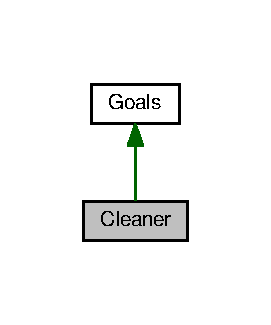
\includegraphics[width=130pt]{classCleaner__inherit__graph}
\end{center}
\end{figure}


Collaboration diagram for Cleaner\+:\nopagebreak
\begin{figure}[H]
\begin{center}
\leavevmode
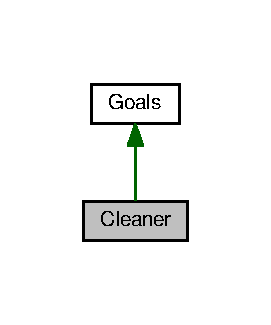
\includegraphics[width=130pt]{classCleaner__coll__graph}
\end{center}
\end{figure}
\subsection*{Public Member Functions}
\begin{DoxyCompactItemize}
\item 
\hyperlink{classCleaner_a4e08e96dad7293b243e7a6856929e21b}{Cleaner} (const std\+::vector$<$ std\+::vector$<$ double $>$$>$ \&\+\_\+\+Goals)
\begin{DoxyCompactList}\small\item\em Constructor for \hyperlink{classCleaner}{Cleaner} Class Takes Goal Points in \+\_\+\+Goals and stores them in a vetor of vectors named Goal\+\_\+\+Points. \end{DoxyCompactList}\item 
void \hyperlink{classCleaner_a6a742590ac6256a15fcfaf6853fd6a97}{Clean\+\_\+\+Room} ()\hypertarget{classCleaner_a6a742590ac6256a15fcfaf6853fd6a97}{}\label{classCleaner_a6a742590ac6256a15fcfaf6853fd6a97}

\begin{DoxyCompactList}\small\item\em Clean\+\_\+\+Room Initializes action client to communicate with move\+\_\+base This function sends goals to move\+\_\+base. \end{DoxyCompactList}\item 
virtual \hyperlink{classCleaner_a86f390999d60ee10a0e53a5946369d9d}{$\sim$\+Cleaner} ()\hypertarget{classCleaner_a86f390999d60ee10a0e53a5946369d9d}{}\label{classCleaner_a86f390999d60ee10a0e53a5946369d9d}

\begin{DoxyCompactList}\small\item\em Destructor for \hyperlink{classCleaner}{Cleaner} Class. \end{DoxyCompactList}\end{DoxyCompactItemize}
\subsection*{Additional Inherited Members}


\subsection{Detailed Description}
\hyperlink{classCleaner}{Cleaner} class This class is a protected derived class of base class \hyperlink{classGoals}{Goals}. This class contains functions which initialize action client. This class also uses functions from \hyperlink{classGoals}{Goals} class to send goals sequentially to move\+\_\+base. 

\subsection{Constructor \& Destructor Documentation}
\index{Cleaner@{Cleaner}!Cleaner@{Cleaner}}
\index{Cleaner@{Cleaner}!Cleaner@{Cleaner}}
\subsubsection[{\texorpdfstring{Cleaner(const std\+::vector$<$ std\+::vector$<$ double $>$$>$ \&\+\_\+\+Goals)}{Cleaner(const std::vector< std::vector< double >> &_Goals)}}]{\setlength{\rightskip}{0pt plus 5cm}Cleaner\+::\+Cleaner (
\begin{DoxyParamCaption}
\item[{const std\+::vector$<$ std\+::vector$<$ double $>$$>$ \&}]{\+\_\+\+Goals}
\end{DoxyParamCaption}
)\hspace{0.3cm}{\ttfamily [explicit]}}\hypertarget{classCleaner_a4e08e96dad7293b243e7a6856929e21b}{}\label{classCleaner_a4e08e96dad7293b243e7a6856929e21b}


Constructor for \hyperlink{classCleaner}{Cleaner} Class Takes Goal Points in \+\_\+\+Goals and stores them in a vetor of vectors named Goal\+\_\+\+Points. 


\begin{DoxyParams}{Parameters}
{\em \+\_\+\+Goals} & vector of vectors of type double \\
\hline
\end{DoxyParams}


The documentation for this class was generated from the following files\+:\begin{DoxyCompactItemize}
\item 
include/\hyperlink{Cleaner_8h}{Cleaner.\+h}\item 
src/\hyperlink{Cleaner_8cpp}{Cleaner.\+cpp}\end{DoxyCompactItemize}

\hypertarget{classGoals}{}\section{Goals Class Reference}
\label{classGoals}\index{Goals@{Goals}}


\hyperlink{classGoals}{Goals} class This class is a base class which contains general use functions. This class contains functions which sets goal point\textquotesingle{}s X,Y,orientation.  




{\ttfamily \#include $<$Goals.\+h$>$}



Inheritance diagram for Goals\+:\nopagebreak
\begin{figure}[H]
\begin{center}
\leavevmode
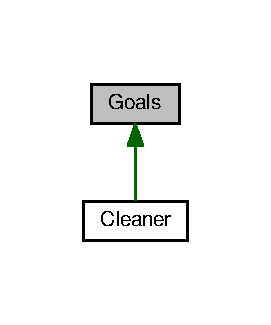
\includegraphics[width=130pt]{classGoals__inherit__graph}
\end{center}
\end{figure}
\subsection*{Public Member Functions}
\begin{DoxyCompactItemize}
\item 
\hyperlink{classGoals_a6b686b508f96f56d28ab0c1f8c15f5b2}{Goals} ()\hypertarget{classGoals_a6b686b508f96f56d28ab0c1f8c15f5b2}{}\label{classGoals_a6b686b508f96f56d28ab0c1f8c15f5b2}

\begin{DoxyCompactList}\small\item\em Constructor for \hyperlink{classGoals}{Goals} Class. \end{DoxyCompactList}\item 
double \hyperlink{classGoals_a587309b801df2c5c805e3c8c1bfddfea}{Set\+\_\+\+Current\+\_\+X} (std\+::vector$<$ double $>$ \&Next\+\_\+\+Goal, move\+\_\+base\+\_\+msgs\+::\+Move\+Base\+Goal \&goal\+\_\+point)
\begin{DoxyCompactList}\small\item\em Set\+\_\+\+Current\+\_\+X a function to set goal\textquotesingle{}s X coordinate. This function sets the goal\textquotesingle{}s X coordinate when given a goal point. \end{DoxyCompactList}\item 
double \hyperlink{classGoals_a815209daf633d7a3a64a1a3a5605cdd0}{Set\+\_\+\+Current\+\_\+Y} (std\+::vector$<$ double $>$ \&Next\+\_\+\+Goal, move\+\_\+base\+\_\+msgs\+::\+Move\+Base\+Goal \&goal\+\_\+point)
\begin{DoxyCompactList}\small\item\em Set\+\_\+\+Current\+\_\+Y a function to set goal\textquotesingle{}s Y coordinate. This function sets the goal\textquotesingle{}s Y coordinate when given a goal point. \end{DoxyCompactList}\item 
virtual \hyperlink{classGoals_a3a48604490cad549dfbb30fbedbf3d54}{$\sim$\+Goals} ()\hypertarget{classGoals_a3a48604490cad549dfbb30fbedbf3d54}{}\label{classGoals_a3a48604490cad549dfbb30fbedbf3d54}

\begin{DoxyCompactList}\small\item\em Destructor for \hyperlink{classGoals}{Goals} Class. \end{DoxyCompactList}\end{DoxyCompactItemize}
\subsection*{Public Attributes}
\begin{DoxyCompactItemize}
\item 
std\+::vector$<$ double $>$ \hyperlink{classGoals_a55d63f2dacadc111b312e6f22f7a33ba}{Get\+\_\+\+Goal}
\end{DoxyCompactItemize}
\subsection*{Protected Member Functions}
\begin{DoxyCompactItemize}
\item 
void \hyperlink{classGoals_a1aded121d6fdcad38f627b46961b58d0}{Set\+\_\+\+Current\+\_\+\+Orientation} (std\+::vector$<$ double $>$ \&Next\+\_\+\+Goal, move\+\_\+base\+\_\+msgs\+::\+Move\+Base\+Goal \&goal\+\_\+point)
\begin{DoxyCompactList}\small\item\em Set\+\_\+\+Current\+\_\+\+Orientation a function to set goal\textquotesingle{}s Orientation. This function sets the goal\textquotesingle{}s orientation when given a goal point. \end{DoxyCompactList}\end{DoxyCompactItemize}
\subsection*{Protected Attributes}
\begin{DoxyCompactItemize}
\item 
std\+::vector$<$ std\+::vector$<$ double $>$ $>$ \hyperlink{classGoals_ad6033ccf299d860e3d5bb826ea5a8bb6}{Goal\+\_\+\+Points}
\end{DoxyCompactItemize}


\subsection{Detailed Description}
\hyperlink{classGoals}{Goals} class This class is a base class which contains general use functions. This class contains functions which sets goal point\textquotesingle{}s X,Y,orientation. 

\subsection{Member Function Documentation}
\index{Goals@{Goals}!Set\+\_\+\+Current\+\_\+\+Orientation@{Set\+\_\+\+Current\+\_\+\+Orientation}}
\index{Set\+\_\+\+Current\+\_\+\+Orientation@{Set\+\_\+\+Current\+\_\+\+Orientation}!Goals@{Goals}}
\subsubsection[{\texorpdfstring{Set\+\_\+\+Current\+\_\+\+Orientation(std\+::vector$<$ double $>$ \&\+Next\+\_\+\+Goal, move\+\_\+base\+\_\+msgs\+::\+Move\+Base\+Goal \&goal\+\_\+point)}{Set_Current_Orientation(std::vector< double > &Next_Goal, move_base_msgs::MoveBaseGoal &goal_point)}}]{\setlength{\rightskip}{0pt plus 5cm}void Goals\+::\+Set\+\_\+\+Current\+\_\+\+Orientation (
\begin{DoxyParamCaption}
\item[{std\+::vector$<$ double $>$ \&}]{Next\+\_\+\+Goal, }
\item[{move\+\_\+base\+\_\+msgs\+::\+Move\+Base\+Goal \&}]{goal\+\_\+point}
\end{DoxyParamCaption}
)\hspace{0.3cm}{\ttfamily [protected]}}\hypertarget{classGoals_a1aded121d6fdcad38f627b46961b58d0}{}\label{classGoals_a1aded121d6fdcad38f627b46961b58d0}


Set\+\_\+\+Current\+\_\+\+Orientation a function to set goal\textquotesingle{}s Orientation. This function sets the goal\textquotesingle{}s orientation when given a goal point. 


\begin{DoxyParams}{Parameters}
{\em Next\+\_\+\+Goal} & is a Goal point of type double vector. \\
\hline
{\em goal\+\_\+point} & is a message of type move\+\_\+base\+\_\+msgs\+::\+Move\+Base\+Goal \\
\hline
\end{DoxyParams}
\index{Goals@{Goals}!Set\+\_\+\+Current\+\_\+X@{Set\+\_\+\+Current\+\_\+X}}
\index{Set\+\_\+\+Current\+\_\+X@{Set\+\_\+\+Current\+\_\+X}!Goals@{Goals}}
\subsubsection[{\texorpdfstring{Set\+\_\+\+Current\+\_\+\+X(std\+::vector$<$ double $>$ \&\+Next\+\_\+\+Goal, move\+\_\+base\+\_\+msgs\+::\+Move\+Base\+Goal \&goal\+\_\+point)}{Set_Current_X(std::vector< double > &Next_Goal, move_base_msgs::MoveBaseGoal &goal_point)}}]{\setlength{\rightskip}{0pt plus 5cm}double Goals\+::\+Set\+\_\+\+Current\+\_\+X (
\begin{DoxyParamCaption}
\item[{std\+::vector$<$ double $>$ \&}]{Next\+\_\+\+Goal, }
\item[{move\+\_\+base\+\_\+msgs\+::\+Move\+Base\+Goal \&}]{goal\+\_\+point}
\end{DoxyParamCaption}
)}\hypertarget{classGoals_a587309b801df2c5c805e3c8c1bfddfea}{}\label{classGoals_a587309b801df2c5c805e3c8c1bfddfea}


Set\+\_\+\+Current\+\_\+X a function to set goal\textquotesingle{}s X coordinate. This function sets the goal\textquotesingle{}s X coordinate when given a goal point. 


\begin{DoxyParams}{Parameters}
{\em Next\+\_\+\+Goal} & is a Goal point of type double vector. \\
\hline
{\em goal\+\_\+point} & is a message of type move\+\_\+base\+\_\+msgs\+::\+Move\+Base\+Goal \\
\hline
\end{DoxyParams}
\begin{DoxyReturn}{Returns}
double type Goal Point\textquotesingle{}s X coordinate. 
\end{DoxyReturn}
\index{Goals@{Goals}!Set\+\_\+\+Current\+\_\+Y@{Set\+\_\+\+Current\+\_\+Y}}
\index{Set\+\_\+\+Current\+\_\+Y@{Set\+\_\+\+Current\+\_\+Y}!Goals@{Goals}}
\subsubsection[{\texorpdfstring{Set\+\_\+\+Current\+\_\+\+Y(std\+::vector$<$ double $>$ \&\+Next\+\_\+\+Goal, move\+\_\+base\+\_\+msgs\+::\+Move\+Base\+Goal \&goal\+\_\+point)}{Set_Current_Y(std::vector< double > &Next_Goal, move_base_msgs::MoveBaseGoal &goal_point)}}]{\setlength{\rightskip}{0pt plus 5cm}double Goals\+::\+Set\+\_\+\+Current\+\_\+Y (
\begin{DoxyParamCaption}
\item[{std\+::vector$<$ double $>$ \&}]{Next\+\_\+\+Goal, }
\item[{move\+\_\+base\+\_\+msgs\+::\+Move\+Base\+Goal \&}]{goal\+\_\+point}
\end{DoxyParamCaption}
)}\hypertarget{classGoals_a815209daf633d7a3a64a1a3a5605cdd0}{}\label{classGoals_a815209daf633d7a3a64a1a3a5605cdd0}


Set\+\_\+\+Current\+\_\+Y a function to set goal\textquotesingle{}s Y coordinate. This function sets the goal\textquotesingle{}s Y coordinate when given a goal point. 


\begin{DoxyParams}{Parameters}
{\em Next\+\_\+\+Goal} & is a Goal point of type double vector. \\
\hline
{\em goal\+\_\+point} & is a message of type move\+\_\+base\+\_\+msgs\+::\+Move\+Base\+Goal \\
\hline
\end{DoxyParams}
\begin{DoxyReturn}{Returns}
double type Goal Point\textquotesingle{}s Y coordinate. 
\end{DoxyReturn}


\subsection{Member Data Documentation}
\index{Goals@{Goals}!Get\+\_\+\+Goal@{Get\+\_\+\+Goal}}
\index{Get\+\_\+\+Goal@{Get\+\_\+\+Goal}!Goals@{Goals}}
\subsubsection[{\texorpdfstring{Get\+\_\+\+Goal}{Get_Goal}}]{\setlength{\rightskip}{0pt plus 5cm}std\+::vector$<$double$>$ Goals\+::\+Get\+\_\+\+Goal}\hypertarget{classGoals_a55d63f2dacadc111b312e6f22f7a33ba}{}\label{classGoals_a55d63f2dacadc111b312e6f22f7a33ba}
Get\+\_\+\+Goal of type double vector, Stores Current Goal Point Data \index{Goals@{Goals}!Goal\+\_\+\+Points@{Goal\+\_\+\+Points}}
\index{Goal\+\_\+\+Points@{Goal\+\_\+\+Points}!Goals@{Goals}}
\subsubsection[{\texorpdfstring{Goal\+\_\+\+Points}{Goal_Points}}]{\setlength{\rightskip}{0pt plus 5cm}std\+::vector$<$std\+::vector$<$double$>$ $>$ Goals\+::\+Goal\+\_\+\+Points\hspace{0.3cm}{\ttfamily [protected]}}\hypertarget{classGoals_ad6033ccf299d860e3d5bb826ea5a8bb6}{}\label{classGoals_ad6033ccf299d860e3d5bb826ea5a8bb6}
Goal\+\_\+\+Points of type vector of double vectors, Stores all Goal Points 

The documentation for this class was generated from the following files\+:\begin{DoxyCompactItemize}
\item 
include/\hyperlink{Goals_8h}{Goals.\+h}\item 
src/\hyperlink{Goals_8cpp}{Goals.\+cpp}\end{DoxyCompactItemize}

\chapter{File Documentation}
\hypertarget{Cleaner_8h}{}\section{include/\+Cleaner.h File Reference}
\label{Cleaner_8h}\index{include/\+Cleaner.\+h@{include/\+Cleaner.\+h}}


This file contains function declarations for \hyperlink{classCleaner}{Cleaner} class.  


{\ttfamily \#include \char`\"{}Goals.\+h\char`\"{}}\\*
{\ttfamily \#include $<$vector$>$}\\*
Include dependency graph for Cleaner.\+h\+:\nopagebreak
\begin{figure}[H]
\begin{center}
\leavevmode
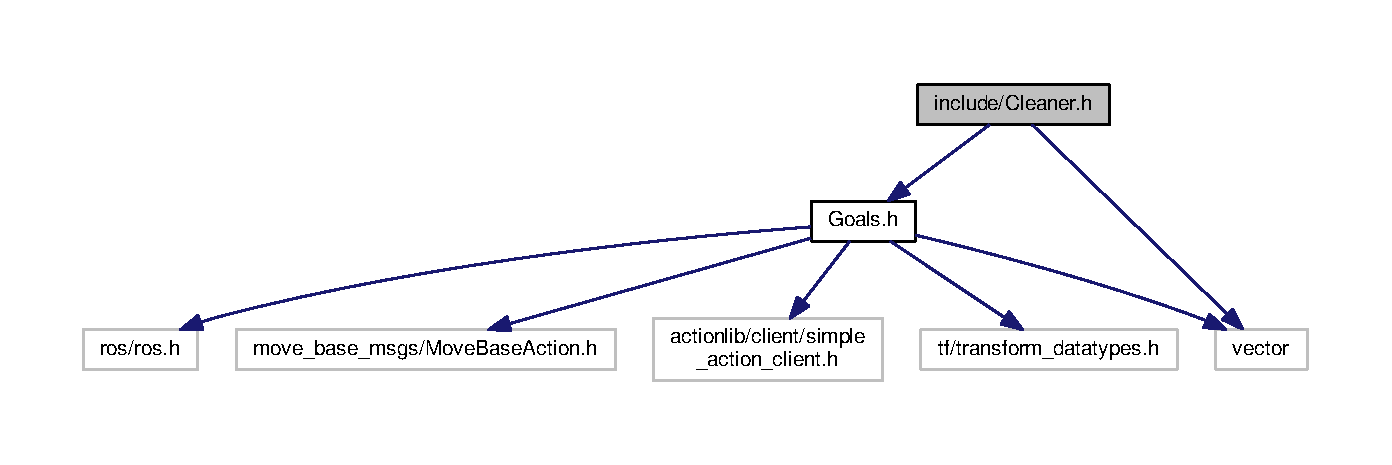
\includegraphics[width=350pt]{Cleaner_8h__incl}
\end{center}
\end{figure}
This graph shows which files directly or indirectly include this file\+:\nopagebreak
\begin{figure}[H]
\begin{center}
\leavevmode
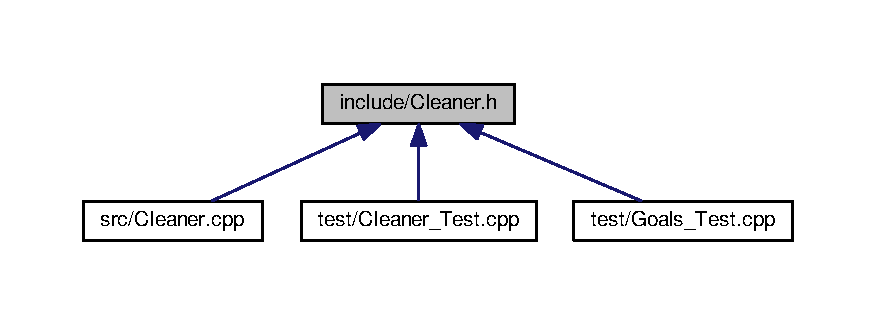
\includegraphics[width=350pt]{Cleaner_8h__dep__incl}
\end{center}
\end{figure}
\subsection*{Classes}
\begin{DoxyCompactItemize}
\item 
class \hyperlink{classCleaner}{Cleaner}
\begin{DoxyCompactList}\small\item\em \hyperlink{classCleaner}{Cleaner} class This class is a protected derived class of base class \hyperlink{classGoals}{Goals}. This class contains functions which initialize action client. This class also uses functions from \hyperlink{classGoals}{Goals} class to send goals sequentially to move\+\_\+base. \end{DoxyCompactList}\end{DoxyCompactItemize}


\subsection{Detailed Description}
This file contains function declarations for \hyperlink{classCleaner}{Cleaner} class. 

\begin{DoxyAuthor}{Author}
Vaibhav Bhilare 
\end{DoxyAuthor}
\begin{DoxyCopyright}{Copyright}
2017, Vaibhav Bhilare
\end{DoxyCopyright}
M\+IT License Copyright (c) 2017 Vaibhav Bhilare

Permission is hereby granted, free of charge, to any person obtaining a copy of this software and associated documentation files (the \char`\"{}\+Software\char`\"{}), to deal in the Software without restriction, including without limitation the rights to use, copy, modify, merge, publish, distribute, sublicense, and/or sell copies of the Software, and to permit persons to whom the Software is furnished to do so, subject to the following conditions\+:

The above copyright notice and this permission notice shall be included in all copies or substantial portions of the Software.

T\+HE S\+O\+F\+T\+W\+A\+RE IS P\+R\+O\+V\+I\+D\+ED \char`\"{}\+A\+S I\+S\char`\"{}, W\+I\+T\+H\+O\+UT W\+A\+R\+R\+A\+N\+TY OF A\+NY K\+I\+ND, E\+X\+P\+R\+E\+SS OR I\+M\+P\+L\+I\+ED, I\+N\+C\+L\+U\+D\+I\+NG B\+UT N\+OT L\+I\+M\+I\+T\+ED TO T\+HE W\+A\+R\+R\+A\+N\+T\+I\+ES OF M\+E\+R\+C\+H\+A\+N\+T\+A\+B\+I\+L\+I\+TY, F\+I\+T\+N\+E\+SS F\+OR A P\+A\+R\+T\+I\+C\+U\+L\+AR P\+U\+R\+P\+O\+SE A\+ND N\+O\+N\+I\+N\+F\+R\+I\+N\+G\+E\+M\+E\+NT. IN NO E\+V\+E\+NT S\+H\+A\+LL T\+HE A\+U\+T\+H\+O\+RS OR C\+O\+P\+Y\+R\+I\+G\+HT H\+O\+L\+D\+E\+RS BE L\+I\+A\+B\+LE F\+OR A\+NY C\+L\+A\+IM, D\+A\+M\+A\+G\+ES OR O\+T\+H\+ER L\+I\+A\+B\+I\+L\+I\+TY, W\+H\+E\+T\+H\+ER IN AN A\+C\+T\+I\+ON OF C\+O\+N\+T\+R\+A\+CT, T\+O\+RT OR O\+T\+H\+E\+R\+W\+I\+SE, A\+R\+I\+S\+I\+NG F\+R\+OM, O\+UT OF OR IN C\+O\+N\+N\+E\+C\+T\+I\+ON W\+I\+TH T\+HE S\+O\+F\+T\+W\+A\+RE OR T\+HE U\+SE OR O\+T\+H\+ER D\+E\+A\+L\+I\+N\+GS IN T\+HE S\+O\+F\+T\+W\+A\+RE. 
\hypertarget{Goals_8h}{}\section{include/\+Goals.h File Reference}
\label{Goals_8h}\index{include/\+Goals.\+h@{include/\+Goals.\+h}}


This file contains function declarations for \hyperlink{classGoals}{Goals} class.  


{\ttfamily \#include $<$ros/ros.\+h$>$}\\*
{\ttfamily \#include $<$move\+\_\+base\+\_\+msgs/\+Move\+Base\+Action.\+h$>$}\\*
{\ttfamily \#include $<$actionlib/client/simple\+\_\+action\+\_\+client.\+h$>$}\\*
{\ttfamily \#include $<$tf/transform\+\_\+datatypes.\+h$>$}\\*
{\ttfamily \#include $<$vector$>$}\\*
Include dependency graph for Goals.\+h\+:\nopagebreak
\begin{figure}[H]
\begin{center}
\leavevmode
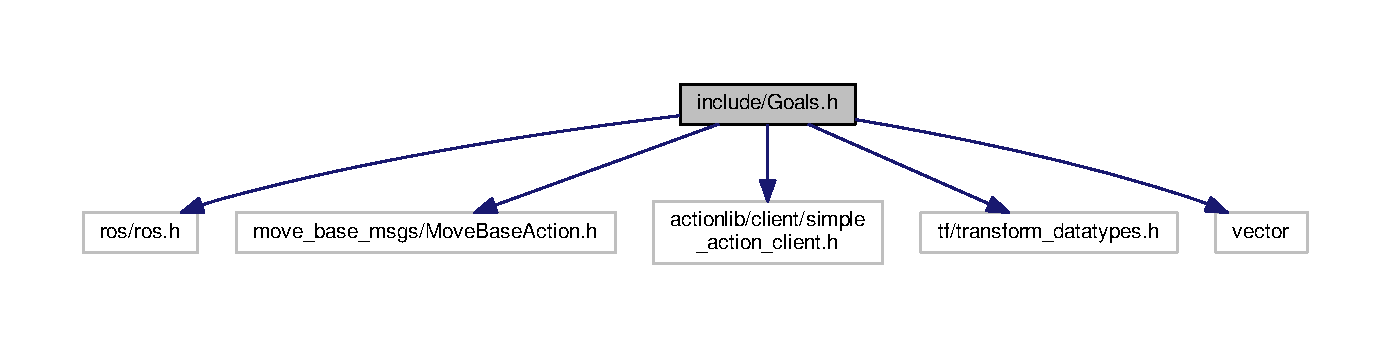
\includegraphics[width=350pt]{Goals_8h__incl}
\end{center}
\end{figure}
This graph shows which files directly or indirectly include this file\+:\nopagebreak
\begin{figure}[H]
\begin{center}
\leavevmode
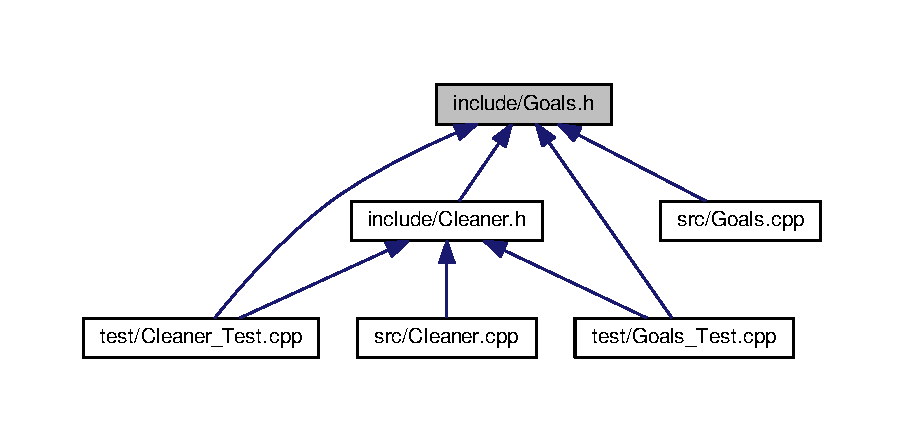
\includegraphics[width=350pt]{Goals_8h__dep__incl}
\end{center}
\end{figure}
\subsection*{Classes}
\begin{DoxyCompactItemize}
\item 
class \hyperlink{classGoals}{Goals}
\begin{DoxyCompactList}\small\item\em \hyperlink{classGoals}{Goals} class This class is a base class which contains general use functions. This class contains functions which sets goal point\textquotesingle{}s X,Y,orientation. \end{DoxyCompactList}\end{DoxyCompactItemize}


\subsection{Detailed Description}
This file contains function declarations for \hyperlink{classGoals}{Goals} class. 

\begin{DoxyAuthor}{Author}
Vaibhav Bhilare 
\end{DoxyAuthor}
\begin{DoxyCopyright}{Copyright}
2017, Vaibhav Bhilare
\end{DoxyCopyright}
M\+IT License Copyright (c) 2017 Vaibhav Bhilare

Permission is hereby granted, free of charge, to any person obtaining a copy of this software and associated documentation files (the \char`\"{}\+Software\char`\"{}), to deal in the Software without restriction, including without limitation the rights to use, copy, modify, merge, publish, distribute, sublicense, and/or sell copies of the Software, and to permit persons to whom the Software is furnished to do so, subject to the following conditions\+:

The above copyright notice and this permission notice shall be included in all copies or substantial portions of the Software.

T\+HE S\+O\+F\+T\+W\+A\+RE IS P\+R\+O\+V\+I\+D\+ED \char`\"{}\+A\+S I\+S\char`\"{}, W\+I\+T\+H\+O\+UT W\+A\+R\+R\+A\+N\+TY OF A\+NY K\+I\+ND, E\+X\+P\+R\+E\+SS OR I\+M\+P\+L\+I\+ED, I\+N\+C\+L\+U\+D\+I\+NG B\+UT N\+OT L\+I\+M\+I\+T\+ED TO T\+HE W\+A\+R\+R\+A\+N\+T\+I\+ES OF M\+E\+R\+C\+H\+A\+N\+T\+A\+B\+I\+L\+I\+TY, F\+I\+T\+N\+E\+SS F\+OR A P\+A\+R\+T\+I\+C\+U\+L\+AR P\+U\+R\+P\+O\+SE A\+ND N\+O\+N\+I\+N\+F\+R\+I\+N\+G\+E\+M\+E\+NT. IN NO E\+V\+E\+NT S\+H\+A\+LL T\+HE A\+U\+T\+H\+O\+RS OR C\+O\+P\+Y\+R\+I\+G\+HT H\+O\+L\+D\+E\+RS BE L\+I\+A\+B\+LE F\+OR A\+NY C\+L\+A\+IM, D\+A\+M\+A\+G\+ES OR O\+T\+H\+ER L\+I\+A\+B\+I\+L\+I\+TY, W\+H\+E\+T\+H\+ER IN AN A\+C\+T\+I\+ON OF C\+O\+N\+T\+R\+A\+CT, T\+O\+RT OR O\+T\+H\+E\+R\+W\+I\+SE, A\+R\+I\+S\+I\+NG F\+R\+OM, O\+UT OF OR IN C\+O\+N\+N\+E\+C\+T\+I\+ON W\+I\+TH T\+HE S\+O\+F\+T\+W\+A\+RE OR T\+HE U\+SE OR O\+T\+H\+ER D\+E\+A\+L\+I\+N\+GS IN T\+HE S\+O\+F\+T\+W\+A\+RE. 
\hypertarget{Cleaner_8cpp}{}\section{src/\+Cleaner.cpp File Reference}
\label{Cleaner_8cpp}\index{src/\+Cleaner.\+cpp@{src/\+Cleaner.\+cpp}}


This file contains function definitions for \hyperlink{classCleaner}{Cleaner} class. This class is dedicated to sending x,y,angle values to move\+\_\+base using functions from \hyperlink{classGoals}{Goals} class.  


{\ttfamily \#include $<$vector$>$}\\*
{\ttfamily \#include \char`\"{}../include/\+Cleaner.\+h\char`\"{}}\\*
Include dependency graph for Cleaner.\+cpp\+:\nopagebreak
\begin{figure}[H]
\begin{center}
\leavevmode
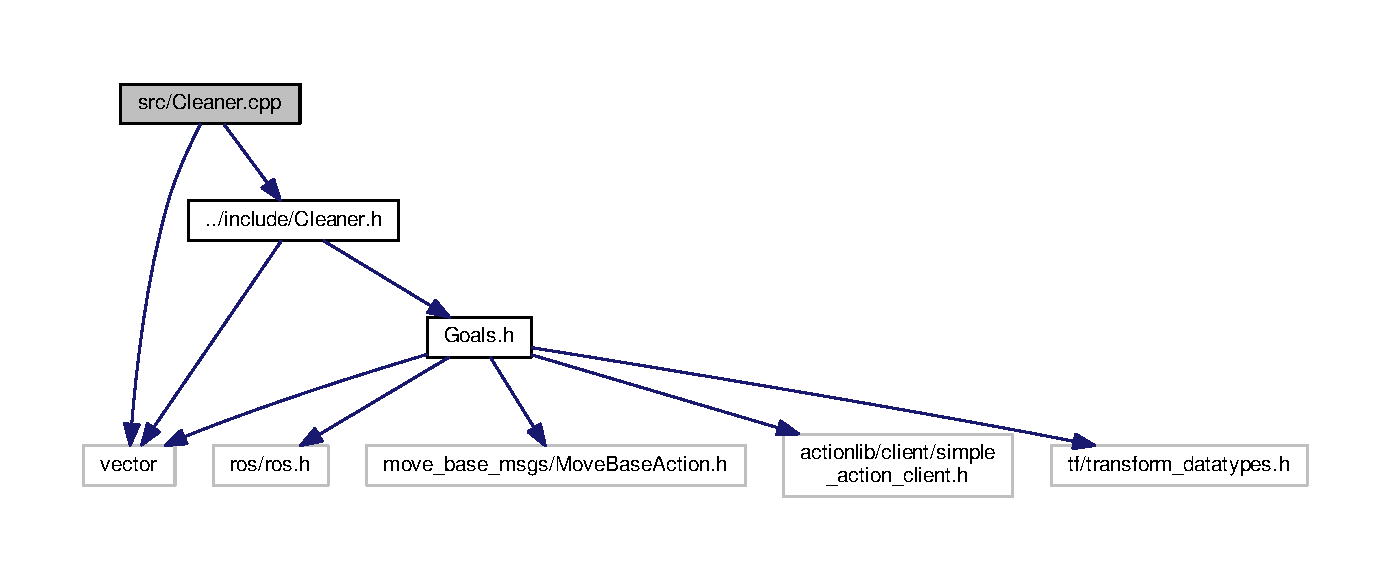
\includegraphics[width=350pt]{Cleaner_8cpp__incl}
\end{center}
\end{figure}


\subsection{Detailed Description}
This file contains function definitions for \hyperlink{classCleaner}{Cleaner} class. This class is dedicated to sending x,y,angle values to move\+\_\+base using functions from \hyperlink{classGoals}{Goals} class. 

\begin{DoxyAuthor}{Author}
Vaibhav Bhilare 
\end{DoxyAuthor}
\begin{DoxyCopyright}{Copyright}
2017, Vaibhav Bhilare
\end{DoxyCopyright}
M\+IT License Copyright (c) 2017 Vaibhav Bhilare

Permission is hereby granted, free of charge, to any person obtaining a copy of this software and associated documentation files (the \char`\"{}\+Software\char`\"{}), to deal in the Software without restriction, including without limitation the rights to use, copy, modify, merge, publish, distribute, sublicense, and/or sell copies of the Software, and to permit persons to whom the Software is furnished to do so, subject to the following conditions\+:

The above copyright notice and this permission notice shall be included in all copies or substantial portions of the Software.

T\+HE S\+O\+F\+T\+W\+A\+RE IS P\+R\+O\+V\+I\+D\+ED \char`\"{}\+A\+S I\+S\char`\"{}, W\+I\+T\+H\+O\+UT W\+A\+R\+R\+A\+N\+TY OF A\+NY K\+I\+ND, E\+X\+P\+R\+E\+SS OR I\+M\+P\+L\+I\+ED, I\+N\+C\+L\+U\+D\+I\+NG B\+UT N\+OT L\+I\+M\+I\+T\+ED TO T\+HE W\+A\+R\+R\+A\+N\+T\+I\+ES OF M\+E\+R\+C\+H\+A\+N\+T\+A\+B\+I\+L\+I\+TY, F\+I\+T\+N\+E\+SS F\+OR A P\+A\+R\+T\+I\+C\+U\+L\+AR P\+U\+R\+P\+O\+SE A\+ND N\+O\+N\+I\+N\+F\+R\+I\+N\+G\+E\+M\+E\+NT. IN NO E\+V\+E\+NT S\+H\+A\+LL T\+HE A\+U\+T\+H\+O\+RS OR C\+O\+P\+Y\+R\+I\+G\+HT H\+O\+L\+D\+E\+RS BE L\+I\+A\+B\+LE F\+OR A\+NY C\+L\+A\+IM, D\+A\+M\+A\+G\+ES OR O\+T\+H\+ER L\+I\+A\+B\+I\+L\+I\+TY, W\+H\+E\+T\+H\+ER IN AN A\+C\+T\+I\+ON OF C\+O\+N\+T\+R\+A\+CT, T\+O\+RT OR O\+T\+H\+E\+R\+W\+I\+SE, A\+R\+I\+S\+I\+NG F\+R\+OM, O\+UT OF OR IN C\+O\+N\+N\+E\+C\+T\+I\+ON W\+I\+TH T\+HE S\+O\+F\+T\+W\+A\+RE OR T\+HE U\+SE OR O\+T\+H\+ER D\+E\+A\+L\+I\+N\+GS IN T\+HE S\+O\+F\+T\+W\+A\+RE. 
\hypertarget{Goals_8cpp}{}\section{src/\+Goals.cpp File Reference}
\label{Goals_8cpp}\index{src/\+Goals.\+cpp@{src/\+Goals.\+cpp}}


This file contains function definitions for \hyperlink{classGoals}{Goals} class. This class is dedicated to assigning x,y,angle values for move\+\_\+base goals.  


{\ttfamily \#include $<$vector$>$}\\*
{\ttfamily \#include \char`\"{}../include/\+Goals.\+h\char`\"{}}\\*
Include dependency graph for Goals.\+cpp\+:\nopagebreak
\begin{figure}[H]
\begin{center}
\leavevmode
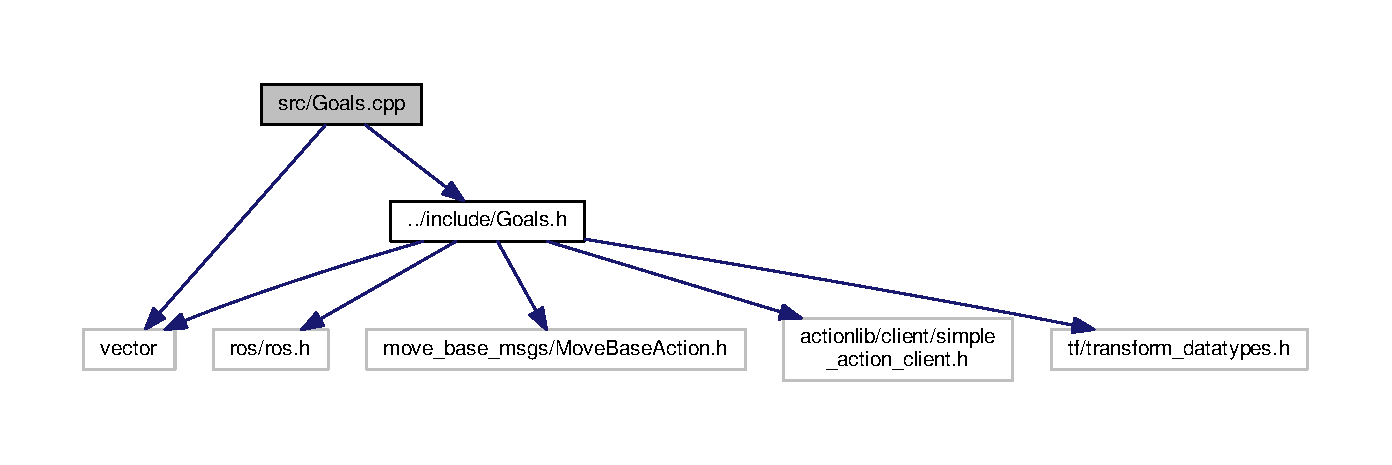
\includegraphics[width=350pt]{Goals_8cpp__incl}
\end{center}
\end{figure}


\subsection{Detailed Description}
This file contains function definitions for \hyperlink{classGoals}{Goals} class. This class is dedicated to assigning x,y,angle values for move\+\_\+base goals. 

\begin{DoxyAuthor}{Author}
Vaibhav Bhilare 
\end{DoxyAuthor}
\begin{DoxyCopyright}{Copyright}
2017, Vaibhav Bhilare
\end{DoxyCopyright}
M\+IT License Copyright (c) 2017 Vaibhav Bhilare

Permission is hereby granted, free of charge, to any person obtaining a copy of this software and associated documentation files (the \char`\"{}\+Software\char`\"{}), to deal in the Software without restriction, including without limitation the rights to use, copy, modify, merge, publish, distribute, sublicense, and/or sell copies of the Software, and to permit persons to whom the Software is furnished to do so, subject to the following conditions\+:

The above copyright notice and this permission notice shall be included in all copies or substantial portions of the Software.

T\+HE S\+O\+F\+T\+W\+A\+RE IS P\+R\+O\+V\+I\+D\+ED \char`\"{}\+A\+S I\+S\char`\"{}, W\+I\+T\+H\+O\+UT W\+A\+R\+R\+A\+N\+TY OF A\+NY K\+I\+ND, E\+X\+P\+R\+E\+SS OR I\+M\+P\+L\+I\+ED, I\+N\+C\+L\+U\+D\+I\+NG B\+UT N\+OT L\+I\+M\+I\+T\+ED TO T\+HE W\+A\+R\+R\+A\+N\+T\+I\+ES OF M\+E\+R\+C\+H\+A\+N\+T\+A\+B\+I\+L\+I\+TY, F\+I\+T\+N\+E\+SS F\+OR A P\+A\+R\+T\+I\+C\+U\+L\+AR P\+U\+R\+P\+O\+SE A\+ND N\+O\+N\+I\+N\+F\+R\+I\+N\+G\+E\+M\+E\+NT. IN NO E\+V\+E\+NT S\+H\+A\+LL T\+HE A\+U\+T\+H\+O\+RS OR C\+O\+P\+Y\+R\+I\+G\+HT H\+O\+L\+D\+E\+RS BE L\+I\+A\+B\+LE F\+OR A\+NY C\+L\+A\+IM, D\+A\+M\+A\+G\+ES OR O\+T\+H\+ER L\+I\+A\+B\+I\+L\+I\+TY, W\+H\+E\+T\+H\+ER IN AN A\+C\+T\+I\+ON OF C\+O\+N\+T\+R\+A\+CT, T\+O\+RT OR O\+T\+H\+E\+R\+W\+I\+SE, A\+R\+I\+S\+I\+NG F\+R\+OM, O\+UT OF OR IN C\+O\+N\+N\+E\+C\+T\+I\+ON W\+I\+TH T\+HE S\+O\+F\+T\+W\+A\+RE OR T\+HE U\+SE OR O\+T\+H\+ER D\+E\+A\+L\+I\+N\+GS IN T\+HE S\+O\+F\+T\+W\+A\+RE. 
\hypertarget{Cleaner__Test_8cpp}{}\section{test/\+Cleaner\+\_\+\+Test.cpp File Reference}
\label{Cleaner__Test_8cpp}\index{test/\+Cleaner\+\_\+\+Test.\+cpp@{test/\+Cleaner\+\_\+\+Test.\+cpp}}


This file contains all tests for \hyperlink{classCleaner}{Cleaner} Class.  


{\ttfamily \#include \char`\"{}../include/\+Cleaner.\+h\char`\"{}}\\*
{\ttfamily \#include $<$gtest/gtest.\+h$>$}\\*
{\ttfamily \#include $<$ros/ros.\+h$>$}\\*
{\ttfamily \#include $<$vector$>$}\\*
{\ttfamily \#include \char`\"{}../include/\+Goals.\+h\char`\"{}}\\*
Include dependency graph for Cleaner\+\_\+\+Test.\+cpp\+:\nopagebreak
\begin{figure}[H]
\begin{center}
\leavevmode
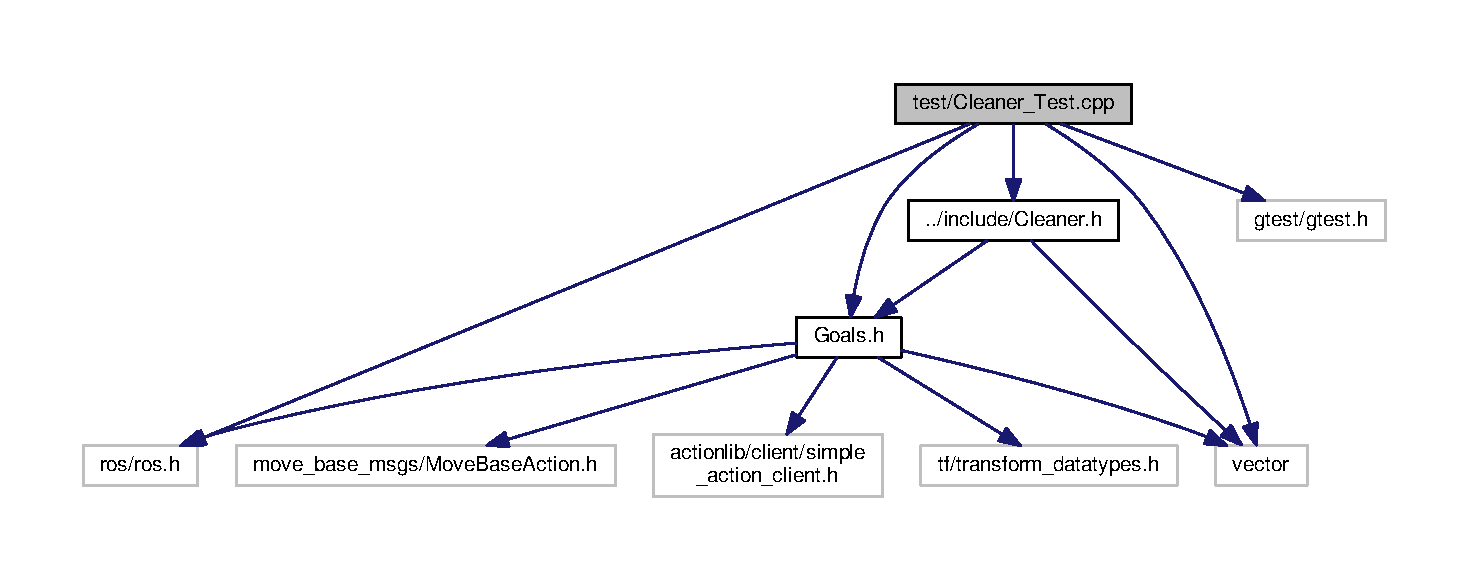
\includegraphics[width=350pt]{Cleaner__Test_8cpp__incl}
\end{center}
\end{figure}
\subsection*{Functions}
\begin{DoxyCompactItemize}
\item 
\hyperlink{Cleaner__Test_8cpp_a481da7bbf384a1c182fc072cd99cafc4}{T\+E\+ST} (T\+E\+S\+T\+Suite, Server\+\_\+\+Existance\+\_\+\+Test)
\begin{DoxyCompactList}\small\item\em Tests whether client comes online when map server is online. \end{DoxyCompactList}\item 
\hyperlink{Cleaner__Test_8cpp_ae6e4fbc2fa3d9199ca781046e97940ba}{T\+E\+ST} (T\+E\+S\+T\+Suite, X\+\_\+\+Test)
\begin{DoxyCompactList}\small\item\em Tests whether the Goal X Point is sent correctly. \end{DoxyCompactList}\item 
\hyperlink{Cleaner__Test_8cpp_a50ec891e18066947a519d2b1c8d130d1}{T\+E\+ST} (T\+E\+S\+T\+Suite, Y\+\_\+\+Test)
\begin{DoxyCompactList}\small\item\em Tests whether the Goal Y Point is Sent correctly. \end{DoxyCompactList}\end{DoxyCompactItemize}


\subsection{Detailed Description}
This file contains all tests for \hyperlink{classCleaner}{Cleaner} Class. 

\begin{DoxyAuthor}{Author}
Vaibhav Bhilare 
\end{DoxyAuthor}
\begin{DoxyCopyright}{Copyright}
2017, Vaibhav Bhilare
\end{DoxyCopyright}
M\+IT License Copyright (c) 2017 Vaibhav Bhilare

Permission is hereby granted, free of charge, to any person obtaining a copy of this software and associated documentation files (the \char`\"{}\+Software\char`\"{}), to deal in the Software without restriction, including without limitation the rights to use, copy, modify, merge, publish, distribute, sublicense, and/or sell copies of the Software, and to permit persons to whom the Software is furnished to do so, subject to the following conditions\+:

The above copyright notice and this permission notice shall be included in all copies or substantial portions of the Software.

T\+HE S\+O\+F\+T\+W\+A\+RE IS P\+R\+O\+V\+I\+D\+ED \char`\"{}\+A\+S I\+S\char`\"{}, W\+I\+T\+H\+O\+UT W\+A\+R\+R\+A\+N\+TY OF A\+NY K\+I\+ND, E\+X\+P\+R\+E\+SS OR I\+M\+P\+L\+I\+ED, I\+N\+C\+L\+U\+D\+I\+NG B\+UT N\+OT L\+I\+M\+I\+T\+ED TO T\+HE W\+A\+R\+R\+A\+N\+T\+I\+ES OF M\+E\+R\+C\+H\+A\+N\+T\+A\+B\+I\+L\+I\+TY, F\+I\+T\+N\+E\+SS F\+OR A P\+A\+R\+T\+I\+C\+U\+L\+AR P\+U\+R\+P\+O\+SE A\+ND N\+O\+N\+I\+N\+F\+R\+I\+N\+G\+E\+M\+E\+NT. IN NO E\+V\+E\+NT S\+H\+A\+LL T\+HE A\+U\+T\+H\+O\+RS OR C\+O\+P\+Y\+R\+I\+G\+HT H\+O\+L\+D\+E\+RS BE L\+I\+A\+B\+LE F\+OR A\+NY C\+L\+A\+IM, D\+A\+M\+A\+G\+ES OR O\+T\+H\+ER L\+I\+A\+B\+I\+L\+I\+TY, W\+H\+E\+T\+H\+ER IN AN A\+C\+T\+I\+ON OF C\+O\+N\+T\+R\+A\+CT, T\+O\+RT OR O\+T\+H\+E\+R\+W\+I\+SE, A\+R\+I\+S\+I\+NG F\+R\+OM, O\+UT OF OR IN C\+O\+N\+N\+E\+C\+T\+I\+ON W\+I\+TH T\+HE S\+O\+F\+T\+W\+A\+RE OR T\+HE U\+SE OR O\+T\+H\+ER D\+E\+A\+L\+I\+N\+GS IN T\+HE S\+O\+F\+T\+W\+A\+RE. 

\subsection{Function Documentation}
\index{Cleaner\+\_\+\+Test.\+cpp@{Cleaner\+\_\+\+Test.\+cpp}!T\+E\+ST@{T\+E\+ST}}
\index{T\+E\+ST@{T\+E\+ST}!Cleaner\+\_\+\+Test.\+cpp@{Cleaner\+\_\+\+Test.\+cpp}}
\subsubsection[{\texorpdfstring{T\+E\+S\+T(\+T\+E\+S\+T\+Suite, Server\+\_\+\+Existance\+\_\+\+Test)}{TEST(TESTSuite, Server_Existance_Test)}}]{\setlength{\rightskip}{0pt plus 5cm}T\+E\+ST (
\begin{DoxyParamCaption}
\item[{T\+E\+S\+T\+Suite}]{, }
\item[{Server\+\_\+\+Existance\+\_\+\+Test}]{}
\end{DoxyParamCaption}
)}\hypertarget{Cleaner__Test_8cpp_a481da7bbf384a1c182fc072cd99cafc4}{}\label{Cleaner__Test_8cpp_a481da7bbf384a1c182fc072cd99cafc4}


Tests whether client comes online when map server is online. 


\begin{DoxyParams}[1]{Parameters}
\mbox{\tt in}  & {\em T\+E\+S\+T\+Suite} & gtest framework \\
\hline
\mbox{\tt in}  & {\em Server\+\_\+\+Existance\+\_\+\+Test} & Test Name \\
\hline
\end{DoxyParams}
\index{Cleaner\+\_\+\+Test.\+cpp@{Cleaner\+\_\+\+Test.\+cpp}!T\+E\+ST@{T\+E\+ST}}
\index{T\+E\+ST@{T\+E\+ST}!Cleaner\+\_\+\+Test.\+cpp@{Cleaner\+\_\+\+Test.\+cpp}}
\subsubsection[{\texorpdfstring{T\+E\+S\+T(\+T\+E\+S\+T\+Suite, X\+\_\+\+Test)}{TEST(TESTSuite, X_Test)}}]{\setlength{\rightskip}{0pt plus 5cm}T\+E\+ST (
\begin{DoxyParamCaption}
\item[{T\+E\+S\+T\+Suite}]{, }
\item[{X\+\_\+\+Test}]{}
\end{DoxyParamCaption}
)}\hypertarget{Cleaner__Test_8cpp_ae6e4fbc2fa3d9199ca781046e97940ba}{}\label{Cleaner__Test_8cpp_ae6e4fbc2fa3d9199ca781046e97940ba}


Tests whether the Goal X Point is sent correctly. 


\begin{DoxyParams}[1]{Parameters}
\mbox{\tt in}  & {\em T\+E\+S\+T\+Suite} & gtest framework \\
\hline
\mbox{\tt in}  & {\em X\+\_\+\+Test} & Test Name \\
\hline
\end{DoxyParams}
\index{Cleaner\+\_\+\+Test.\+cpp@{Cleaner\+\_\+\+Test.\+cpp}!T\+E\+ST@{T\+E\+ST}}
\index{T\+E\+ST@{T\+E\+ST}!Cleaner\+\_\+\+Test.\+cpp@{Cleaner\+\_\+\+Test.\+cpp}}
\subsubsection[{\texorpdfstring{T\+E\+S\+T(\+T\+E\+S\+T\+Suite, Y\+\_\+\+Test)}{TEST(TESTSuite, Y_Test)}}]{\setlength{\rightskip}{0pt plus 5cm}T\+E\+ST (
\begin{DoxyParamCaption}
\item[{T\+E\+S\+T\+Suite}]{, }
\item[{Y\+\_\+\+Test}]{}
\end{DoxyParamCaption}
)}\hypertarget{Cleaner__Test_8cpp_a50ec891e18066947a519d2b1c8d130d1}{}\label{Cleaner__Test_8cpp_a50ec891e18066947a519d2b1c8d130d1}


Tests whether the Goal Y Point is Sent correctly. 


\begin{DoxyParams}[1]{Parameters}
\mbox{\tt in}  & {\em T\+E\+S\+T\+Suite} & gtest framework \\
\hline
\mbox{\tt in}  & {\em Y\+\_\+\+Test} & Test Name \\
\hline
\end{DoxyParams}

\hypertarget{Goals__Test_8cpp}{}\section{test/\+Goals\+\_\+\+Test.cpp File Reference}
\label{Goals__Test_8cpp}\index{test/\+Goals\+\_\+\+Test.\+cpp@{test/\+Goals\+\_\+\+Test.\+cpp}}


This file contains all tests for \hyperlink{classGoals}{Goals} Class.  


{\ttfamily \#include \char`\"{}../include/\+Goals.\+h\char`\"{}}\\*
{\ttfamily \#include $<$gtest/gtest.\+h$>$}\\*
{\ttfamily \#include $<$ros/ros.\+h$>$}\\*
{\ttfamily \#include $<$vector$>$}\\*
{\ttfamily \#include \char`\"{}../include/\+Cleaner.\+h\char`\"{}}\\*
Include dependency graph for Goals\+\_\+\+Test.\+cpp\+:\nopagebreak
\begin{figure}[H]
\begin{center}
\leavevmode
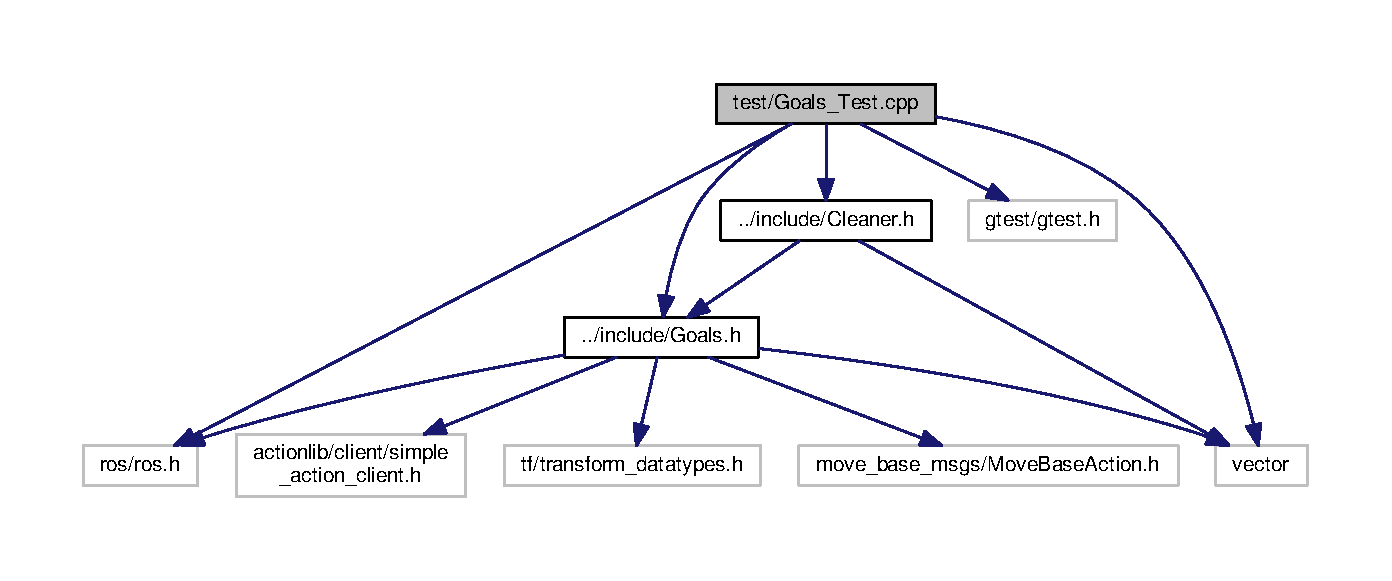
\includegraphics[width=350pt]{Goals__Test_8cpp__incl}
\end{center}
\end{figure}
\subsection*{Functions}
\begin{DoxyCompactItemize}
\item 
\hyperlink{Goals__Test_8cpp_aa7dd8033db68a18ead226c984fe50859}{T\+E\+ST} (T\+E\+S\+T\+Suite, Goal\+\_\+\+Test)
\begin{DoxyCompactList}\small\item\em Tests whether the Goal Point is sent correctly. \end{DoxyCompactList}\item 
\hyperlink{Goals__Test_8cpp_a64e629586c73c12d70b5f39ab07cc819}{T\+E\+ST} (T\+E\+S\+T\+Suite, Goal\+\_\+\+X\+\_\+\+Test)
\begin{DoxyCompactList}\small\item\em Tests whether the Goal X Point is sent correctly. \end{DoxyCompactList}\item 
\hyperlink{Goals__Test_8cpp_a5bfb00edee0344ec668e75c260c8fcdf}{T\+E\+ST} (T\+E\+S\+T\+Suite, Goal\+\_\+\+Y\+\_\+\+Test)
\begin{DoxyCompactList}\small\item\em Tests whether the Goal Y Point is Sent correctly. \end{DoxyCompactList}\end{DoxyCompactItemize}


\subsection{Detailed Description}
This file contains all tests for \hyperlink{classGoals}{Goals} Class. 

\begin{DoxyAuthor}{Author}
Vaibhav Bhilare 
\end{DoxyAuthor}
\begin{DoxyCopyright}{Copyright}
2017, Vaibhav Bhilare
\end{DoxyCopyright}
M\+IT License Copyright (c) 2017 Vaibhav Bhilare

Permission is hereby granted, free of charge, to any person obtaining a copy of this software and associated documentation files (the \char`\"{}\+Software\char`\"{}), to deal in the Software without restriction, including without limitation the rights to use, copy, modify, merge, publish, distribute, sublicense, and/or sell copies of the Software, and to permit persons to whom the Software is furnished to do so, subject to the following conditions\+:

The above copyright notice and this permission notice shall be included in all copies or substantial portions of the Software.

T\+HE S\+O\+F\+T\+W\+A\+RE IS P\+R\+O\+V\+I\+D\+ED \char`\"{}\+A\+S I\+S\char`\"{}, W\+I\+T\+H\+O\+UT W\+A\+R\+R\+A\+N\+TY OF A\+NY K\+I\+ND, E\+X\+P\+R\+E\+SS OR I\+M\+P\+L\+I\+ED, I\+N\+C\+L\+U\+D\+I\+NG B\+UT N\+OT L\+I\+M\+I\+T\+ED TO T\+HE W\+A\+R\+R\+A\+N\+T\+I\+ES OF M\+E\+R\+C\+H\+A\+N\+T\+A\+B\+I\+L\+I\+TY, F\+I\+T\+N\+E\+SS F\+OR A P\+A\+R\+T\+I\+C\+U\+L\+AR P\+U\+R\+P\+O\+SE A\+ND N\+O\+N\+I\+N\+F\+R\+I\+N\+G\+E\+M\+E\+NT. IN NO E\+V\+E\+NT S\+H\+A\+LL T\+HE A\+U\+T\+H\+O\+RS OR C\+O\+P\+Y\+R\+I\+G\+HT H\+O\+L\+D\+E\+RS BE L\+I\+A\+B\+LE F\+OR A\+NY C\+L\+A\+IM, D\+A\+M\+A\+G\+ES OR O\+T\+H\+ER L\+I\+A\+B\+I\+L\+I\+TY, W\+H\+E\+T\+H\+ER IN AN A\+C\+T\+I\+ON OF C\+O\+N\+T\+R\+A\+CT, T\+O\+RT OR O\+T\+H\+E\+R\+W\+I\+SE, A\+R\+I\+S\+I\+NG F\+R\+OM, O\+UT OF OR IN C\+O\+N\+N\+E\+C\+T\+I\+ON W\+I\+TH T\+HE S\+O\+F\+T\+W\+A\+RE OR T\+HE U\+SE OR O\+T\+H\+ER D\+E\+A\+L\+I\+N\+GS IN T\+HE S\+O\+F\+T\+W\+A\+RE. 

\subsection{Function Documentation}
\index{Goals\+\_\+\+Test.\+cpp@{Goals\+\_\+\+Test.\+cpp}!T\+E\+ST@{T\+E\+ST}}
\index{T\+E\+ST@{T\+E\+ST}!Goals\+\_\+\+Test.\+cpp@{Goals\+\_\+\+Test.\+cpp}}
\subsubsection[{\texorpdfstring{T\+E\+S\+T(\+T\+E\+S\+T\+Suite, Goal\+\_\+\+Test)}{TEST(TESTSuite, Goal_Test)}}]{\setlength{\rightskip}{0pt plus 5cm}T\+E\+ST (
\begin{DoxyParamCaption}
\item[{T\+E\+S\+T\+Suite}]{, }
\item[{Goal\+\_\+\+Test}]{}
\end{DoxyParamCaption}
)}\hypertarget{Goals__Test_8cpp_aa7dd8033db68a18ead226c984fe50859}{}\label{Goals__Test_8cpp_aa7dd8033db68a18ead226c984fe50859}


Tests whether the Goal Point is sent correctly. 


\begin{DoxyParams}[1]{Parameters}
\mbox{\tt in}  & {\em T\+E\+S\+T\+Suite} & gtest framework \\
\hline
\mbox{\tt in}  & {\em Goal\+\_\+\+Test} & Test Name \\
\hline
\end{DoxyParams}
\index{Goals\+\_\+\+Test.\+cpp@{Goals\+\_\+\+Test.\+cpp}!T\+E\+ST@{T\+E\+ST}}
\index{T\+E\+ST@{T\+E\+ST}!Goals\+\_\+\+Test.\+cpp@{Goals\+\_\+\+Test.\+cpp}}
\subsubsection[{\texorpdfstring{T\+E\+S\+T(\+T\+E\+S\+T\+Suite, Goal\+\_\+\+X\+\_\+\+Test)}{TEST(TESTSuite, Goal_X_Test)}}]{\setlength{\rightskip}{0pt plus 5cm}T\+E\+ST (
\begin{DoxyParamCaption}
\item[{T\+E\+S\+T\+Suite}]{, }
\item[{Goal\+\_\+\+X\+\_\+\+Test}]{}
\end{DoxyParamCaption}
)}\hypertarget{Goals__Test_8cpp_a64e629586c73c12d70b5f39ab07cc819}{}\label{Goals__Test_8cpp_a64e629586c73c12d70b5f39ab07cc819}


Tests whether the Goal X Point is sent correctly. 


\begin{DoxyParams}[1]{Parameters}
\mbox{\tt in}  & {\em T\+E\+S\+T\+Suite} & gtest framework \\
\hline
\mbox{\tt in}  & {\em Goal\+\_\+\+X\+\_\+\+Test} & Test Name \\
\hline
\end{DoxyParams}
\index{Goals\+\_\+\+Test.\+cpp@{Goals\+\_\+\+Test.\+cpp}!T\+E\+ST@{T\+E\+ST}}
\index{T\+E\+ST@{T\+E\+ST}!Goals\+\_\+\+Test.\+cpp@{Goals\+\_\+\+Test.\+cpp}}
\subsubsection[{\texorpdfstring{T\+E\+S\+T(\+T\+E\+S\+T\+Suite, Goal\+\_\+\+Y\+\_\+\+Test)}{TEST(TESTSuite, Goal_Y_Test)}}]{\setlength{\rightskip}{0pt plus 5cm}T\+E\+ST (
\begin{DoxyParamCaption}
\item[{T\+E\+S\+T\+Suite}]{, }
\item[{Goal\+\_\+\+Y\+\_\+\+Test}]{}
\end{DoxyParamCaption}
)}\hypertarget{Goals__Test_8cpp_a5bfb00edee0344ec668e75c260c8fcdf}{}\label{Goals__Test_8cpp_a5bfb00edee0344ec668e75c260c8fcdf}


Tests whether the Goal Y Point is Sent correctly. 


\begin{DoxyParams}[1]{Parameters}
\mbox{\tt in}  & {\em T\+E\+S\+T\+Suite} & gtest framework \\
\hline
\mbox{\tt in}  & {\em Goal\+\_\+\+Y\+\_\+\+Test} & Test Name \\
\hline
\end{DoxyParams}

%--- End generated contents ---

% Index
\backmatter
\newpage
\phantomsection
\clearemptydoublepage
\addcontentsline{toc}{chapter}{Index}
\printindex

\end{document}
